\chapter{Background}
The algorithms and data structures used in this thesis have been introduced and discussed below.
\section{Word-Vectors by using Skip-Gram}
\label{sec:skipgram}
Mikolov et al. (2013b) proposed two neural network models for building word vectors from large unlabelled corpora; Continuous Bag of Words(CBOW) and Skip-Gram.  In the CBOW model, the context is the input, and one tries to learn a vector for the central word; in Skip grams, the input is the target word and one tries to guess the set of contexts.  The Skip gram was found to perform better on smaller corpora, and here we have focused on this model for building our word vectors. The model uses each current word as an input to a log-linear classifier with continuous projection layer, and predict words within a certain range before and after the current word. The objective is to maximize the probability of the context given a word within a language model:

\begin{center} $p(c|w;\theta)=\frac{\exp^{v_c.v_w}}{\sum_{c' \in C}\exp^{v_c.v_w}}$ \end{center}
where $v_c$ and $v_w$ $\in$ $R^d$ are vector representations for context $c$ and word $w$ respectively. $C$ is the set of all available contexts. The parameters $\theta$ are $v_ci$, $v_wi$ for $w \in V$, $c \in C$, $i \in 1,....,d$ (a total of $|C| \times |V| \times d$ parameters).\\

The weights between the input layer and the output layer can be represented by a $V \times N$ matrix \textbf{W}. Each row of \textbf{W} is the $N$-dimension vector representation $v_w$ of the associated word of the input layer.Given a word, assuming $x_k=1$ and $x_{k'}=0$ for $k' \neq k$, then
\begin{center}
$h=x^TW=W_{(k,.)}:=v_{w_I}$
\end{center}
which is essentially copying the $k$-th row of \textbf{W} to \textbf{h}. $v_{w_I}$ is the vector representation of the input word $w_I$.

From the hidden layer to the output layer, there is a different weight matrix \textbf{W'}=$\{w_{ij}^{'}\}$ which is a $N \times V$ matrix. Then we can use soft-max, a log-linear classification model, to obtain the posterior distribution of words, which is a multinomial distribution.\\
On the output layer, instead of outputing one multinomial distribution, we are outputing C multinomial distributions. Each output is computed using the same hidden$\rightarrow$output matrix.
\begin{center}
$p(w_{c,j}=w_{O,c}|w_I)=y_{c,j}=\frac{exp(u_{c,j})}{\sum_{j'=1}^{V}exp(u_{j'})}$
\end{center}
where $w_{c,j}$ is the $j$-th word on the $c$-th panel of the output layer; $w_{O,c}$ is the actual $c$-th word in the output context words; $w_I$ is the only input word; $y_{c,j}$ is the output of the $j$-th node on the $c$-th panel of the output layer; $u_{c,j}$ is the net input of the $j$-th node on the $c$-th panel of the output layer.
Because the output layer panels share the same weights, thus
\begin{center}
$u_{c,j}=u_j=v`_{w_j}^T.h$, for $c=1,2...,C$
\end{center}
where $v'_{w_j}$ is the output vector of the $j$-th word in the vocabulary, $w_j$, and also $v'_{w_j}$ is taken from a column of the hidden$\rightarrow$output weight matrix, \textbf{W'} .

The loss function is
\begin{center}
E = -$\log p(w_{O,1},w_{O,2},....,w_{O,C}|w_I)$\\
=-$\log \prod_{c=1}^{C}\frac{exp(u_{c,j_{c}^{*	}})}{\sum_{j'=1}^{V}exp(u_{j'})}$\\
=-$\sum_{c=1}^{C} u_{j_{c}^{*}}+C.\log \sum_{j'=1}^{V}exp(u_{j'})$
\end{center}
where $j_{c}^{*}$ is the index of the actual $c$-th output context word in the vocabulary.

After taking the necessary derivatives, the update equation for the hidden$\rightarrow$output weight matrix, \textbf{W'},
\begin{center}
$w'{ij}^{(new)}=w'{ij}^{(old)}-\eta .EI_j.h_i$
\end{center}
or,
\begin{center}
$v'{w_j}^{(new)}=v'{w_j}^{(old)}-\eta .EI_j.\textbf{h}$ for $j=1,2,.....,V$
\end{center}

The update equation for the input$\rightarrow$hidden weight matrix, \textbf{W},
\begin{center}
$v{w_I}^{(new)}=v{w_I}^{(old)}-\eta .EH$
\end{center}
where $EH$ is a $N$-dimensional vector. Its each component is defined as
\begin{center}
$EH_i=\sum_{j=1}^{V}EI_j.w'_{ij}$
\end{center}

\begin{figure}[ht!]
\centering
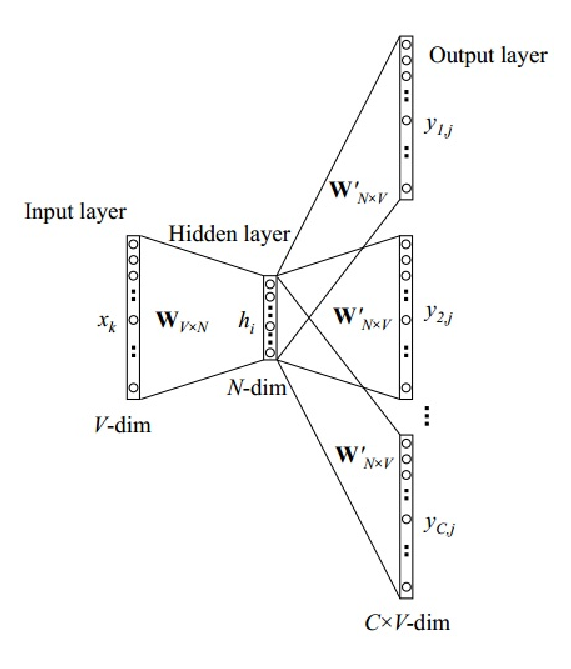
\includegraphics[width=70mm, height=70mm]{skipgram.eps}
\caption{Skip Gram Model(Figure from Rong (2014)) \label{fig:skipgram}}
\end{figure}

\subsection{tf-idf}
\label{subsec:tfidf}
Let $D=d_1, d_2, d_3....d_N$ be $N$ documents under study and $T=t_1, t_2, t_3,....t_M$ be the $M$ unique terms in these documents, then each document can be represented as a $M$-dimensional vector:\\
$t_d=\{tf_1,tf_2,tf_3,...tf_M\}$\\
$tf-idf$ weights discounts the frequency of terms based on their importance to a particular document in the entire document set collection under consideration. This is done as follows:
\begin{center}
$tfidf(d,t)=tf(d,t) \times \log(\frac{|D|}{df(t)})$ 
\end{center}
Here $df(t)$ is the number of documents in which term $t$ appears.

\subsection{Vector Averaging for phrases}
	\label{sec:vectoraveraging}
As an output of the word vector learning, we now have a $n$-dimensional
vector representation for each word in the Hindi corpus.  Now we need to
assign features for sentences and paragraphs taken from the sentiment dataset
(training and test).  Mikolov et al. (2013b) and Levy et al. (2014) show that
many relational similarities can be recovered by means of vector arithmetic
in the embedded space.  Thus, additive models are useful, though
others have claimed that multiplicative models correlate better with human
judgments~\cite{Mitchell:08,Socher:13}.  In this work, we have retained teh
simplicity of vector averaging to model larger chunks of  discourse.
This models the sentence/document in the same high dimensional space.

A preprocessing step involved removing some words that appear at very high or
very low frequencies in the corpus.  
Our model was trained on the Hindi Wikipedia dump to create vector
representations for words. The previous two vectors were concatenated to
create another feature set for training purpose.  
%?? SIZE of wikipedia corpus, number of independent words etc. 

\underline{\emph{Algorithm}}
\begin{enumerate}
%\setlength{\itemsep}{0.5pt}
\item Input the Hindi text corpus
\item Train skip-gram model to obtain word vector representation
\item Given a sentiment training set, obtain average vector data for each sentence/document
\item Obtain tf-idf vector for each sentence/document in the corpus
\item Concatenate vectors of step 3 and step 4 to obtain a feature set for a training instance
\item Train linear SVM with $m$-fold cross validation to create a classifier
(here $m$=20)
\end{enumerate}

\section{Document Vectors}
This distributed representation of sentences and documents~\cite{Le:14} modifies wors2vec (Skip-Gram) algorithm to unsupervised learning of continuous representations for larger blocks of text, such as sentences, paragraphs or entire documents. The algorithm represents each document by a dense vector which is later trained and tuned to predict words in the sentence\/document.\\
In Paragraph Vector framework, every paragraph is mapped to a unique vector and id, represented by a matrix $D$, which is a column matrix. Every word is mapped to a unique vector and word vectors are conactenated or averaged to predict the context, i.e., the next word.\\
The change in this framework is that the $h$(in Skip-Gram model's equation) is now constructed in a different way. It is now constructed using both $W$ and $D$.\\
The contexts are fixed-length and sampled from a sliding window over the paragraph. The paragraph vector is shared across all contexts generated from the same paragraph but not across paragraphs.  The word vector matrix W, however, is shared across paragraphs. i.e., the vector for "good" is the same for all paragraphs.\\

The paragraph vectors and word vectors are trained using stochastic gradient descent and the gradient is obtained via backpropagation.  At every step of stochastic gradient descent, one can sample a fixed-length context from a random paragraph, compute the error gradient from the network in Figure \ref{fig:doc2vec} and use the gradient to update the parameters in our model. At prediction time, one needs to perform an inference step to compute the paragraph vector for a new paragraph. This is also obtained by gradient descent.  In this step, the parameters for the rest of the model, the word vectors W
and the softmax weights, are fixed.

\begin{figure}[ht!]
\centering
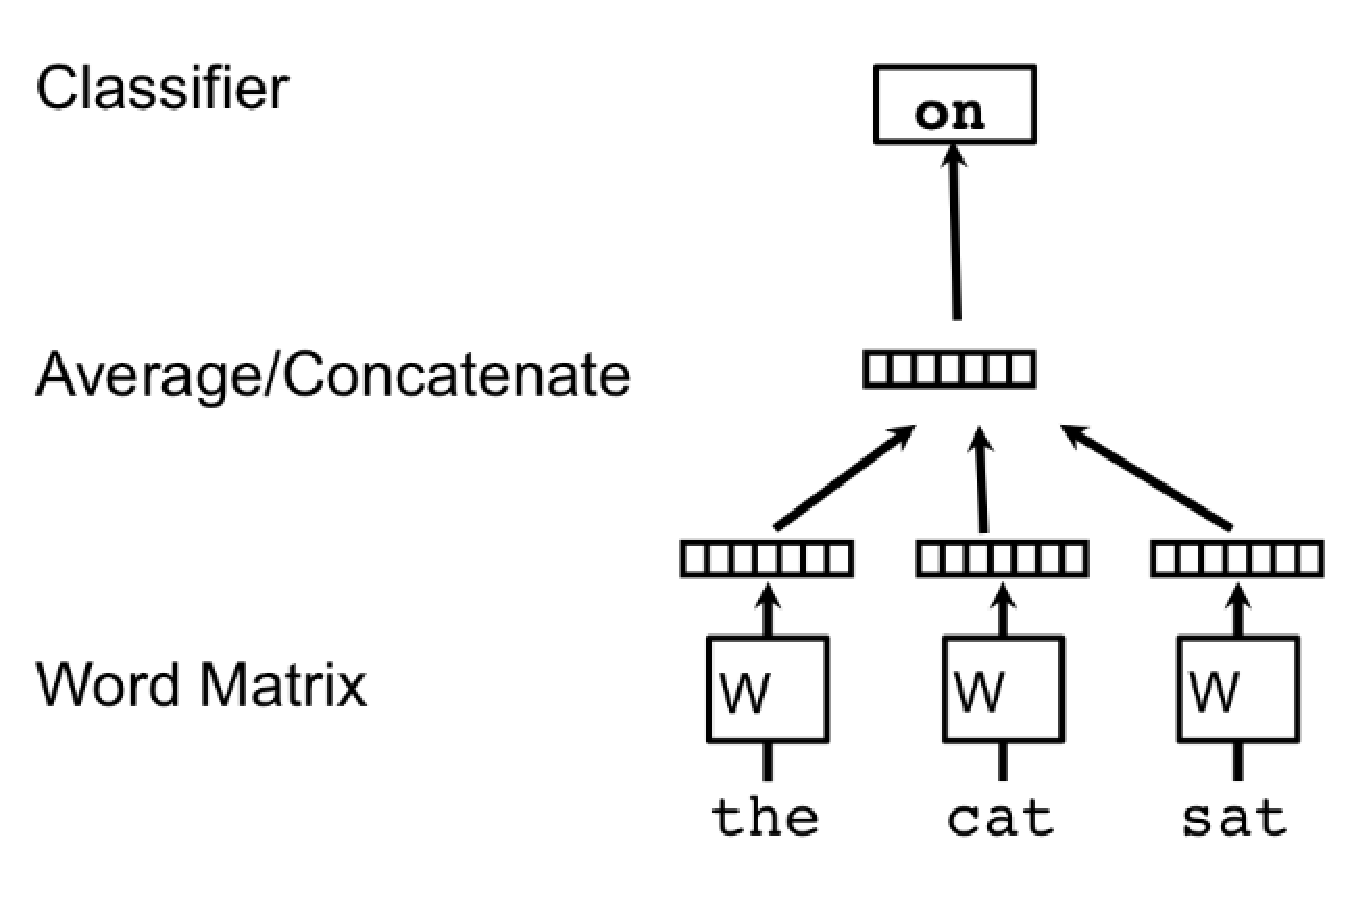
\includegraphics[width=110mm, height=70mm]{doc2vec_word_vector.eps}
\caption{Framework for learning word vectors(Figure from Le (2014)). \label{fig:word2vec}}
\end{figure}
In Figure \ref{fig:word2vec}, context  of three words ("the", "cat" and "sat") is used to predict the fourth word ("on"). The input words are mapped to columns of the matrix $W$ to predict the output word(Figure from Le (2014)).

\begin{figure}[ht!]
\centering
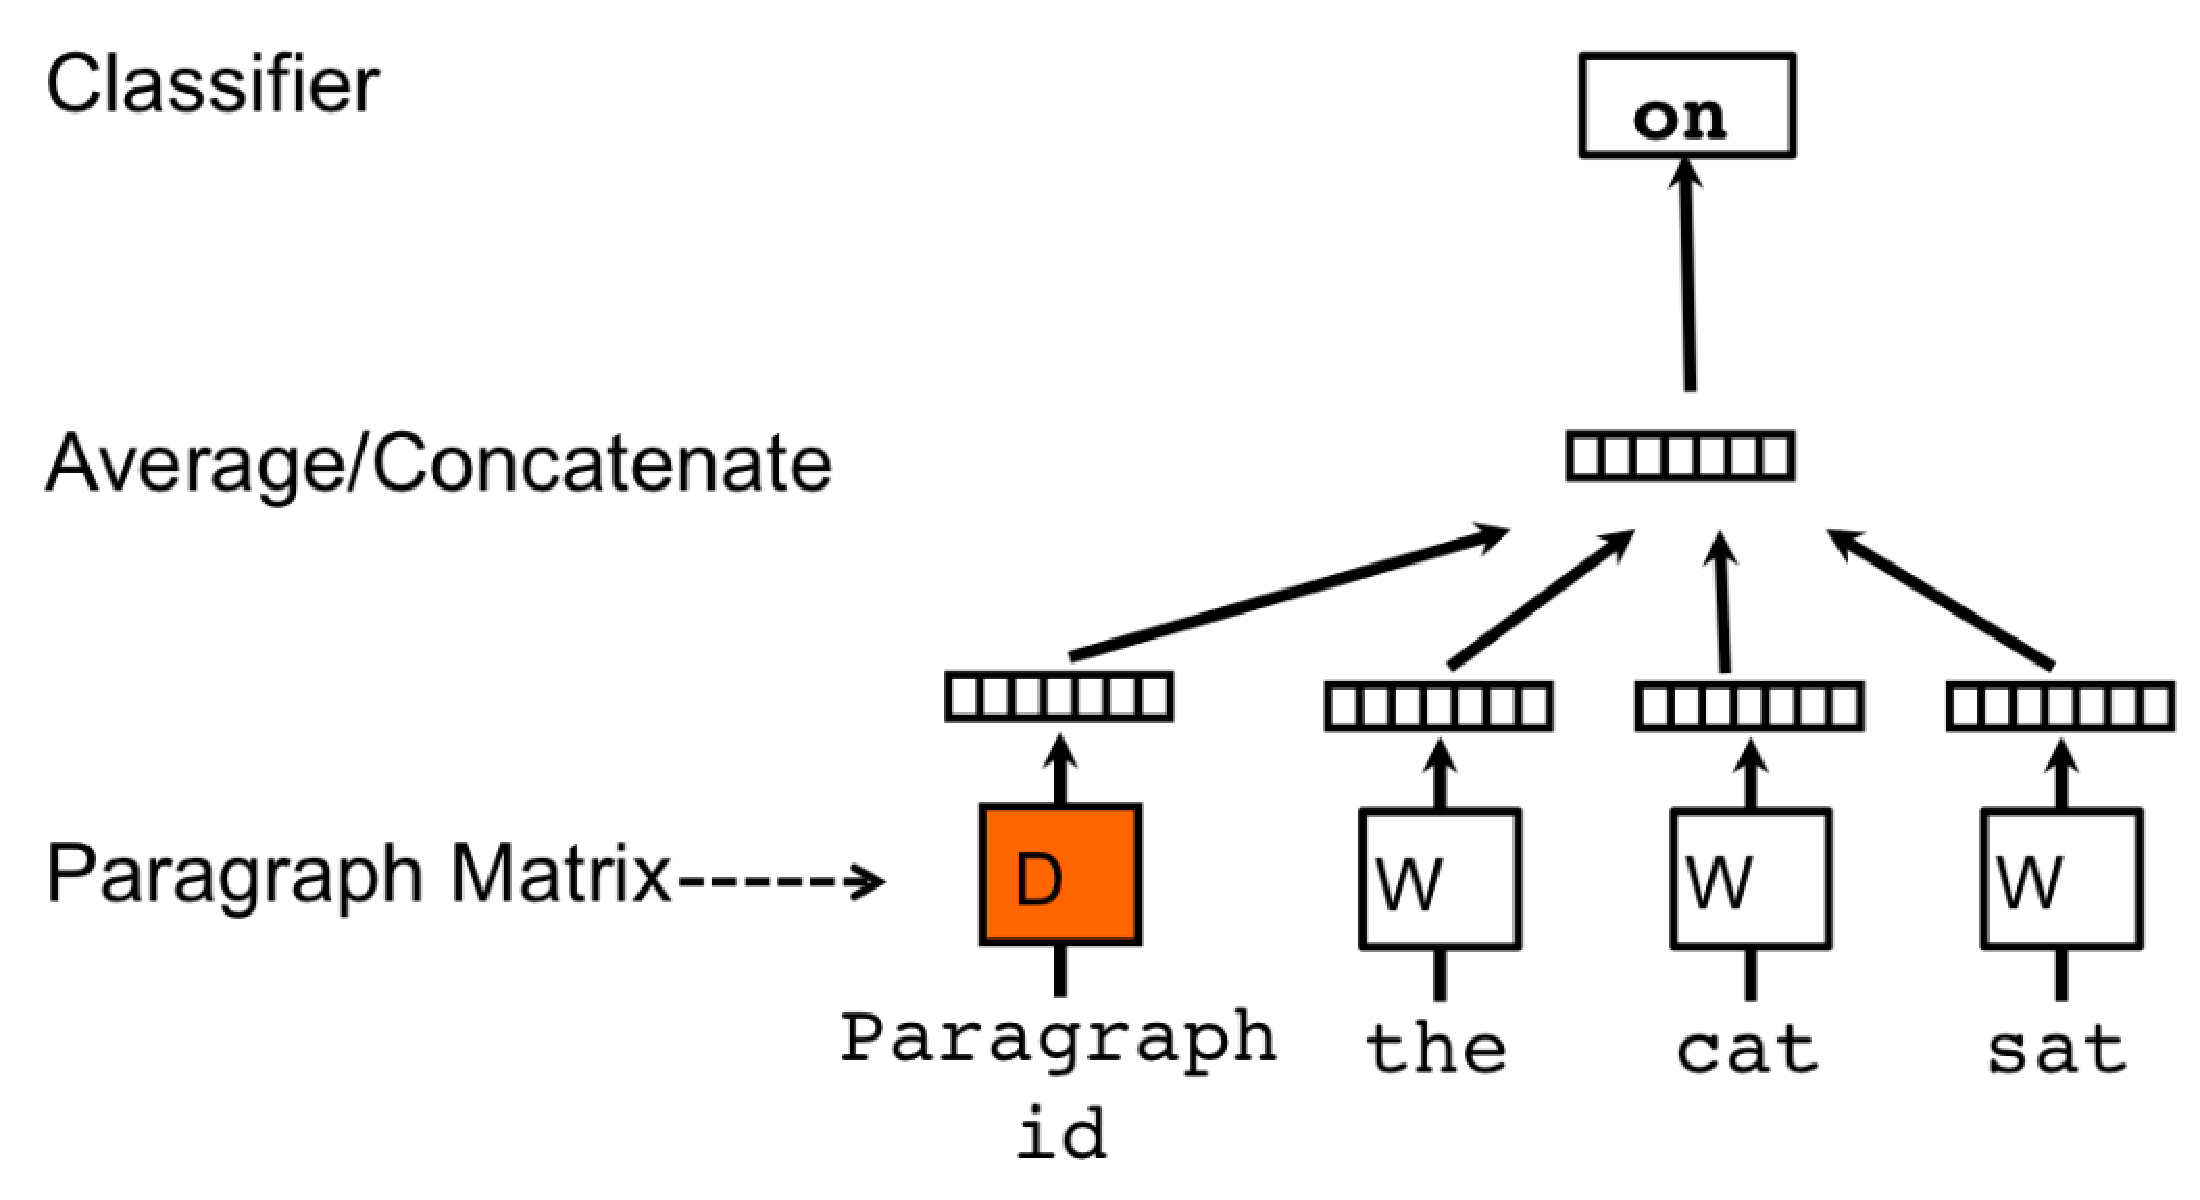
\includegraphics[width=110mm, height=70mm]{doc2vec.eps}
\caption{Framework for learning paragraph vectors(Figure from Le (2014)). \label{fig:doc2vec}}
\end{figure}
In Figure \ref{fig:doc2vec}, the only change is the additional paragraph token that is mapped to a vector via matrix $D$. In this model, the concatenation or average of this vector with a context of three words is used to predict the fourth word. The paragraph vector represents the missing information from the current context and can act as a memory of the topic of the paragraph.

The advantage of using paragraph vectors is that they inherit the propery of word vectors, i.e., the semantics of the words. In addition, they also take into consideration a small context around each word which is in close resemblance to the n-gram model with a large n. This property is crucial because the n-gram model preserves a lot of information of the sentence\/paragraph, which includes the word order also. This model also performs better than the Bag-of-Words model which would create a very high-dimensional representation that has very poor generalization.

\section{Recurrent Neural Network}
\label{sec:rnn}
The primary feature of a Recurrent Network is that it contains atleast one feed-back connection which captures dynamic temporal behavior and allows it to learn sequences. They have application in tasks such as prediction of a word given the context, perform sequence recognition/reproduction.\\
Recurrent Neural Networks have many different forms. One of them is a Fully Recurrent Network, a network of neuron-like units, each with a directed connection to every other unit.\\
\begin{figure}[ht!]
\centering
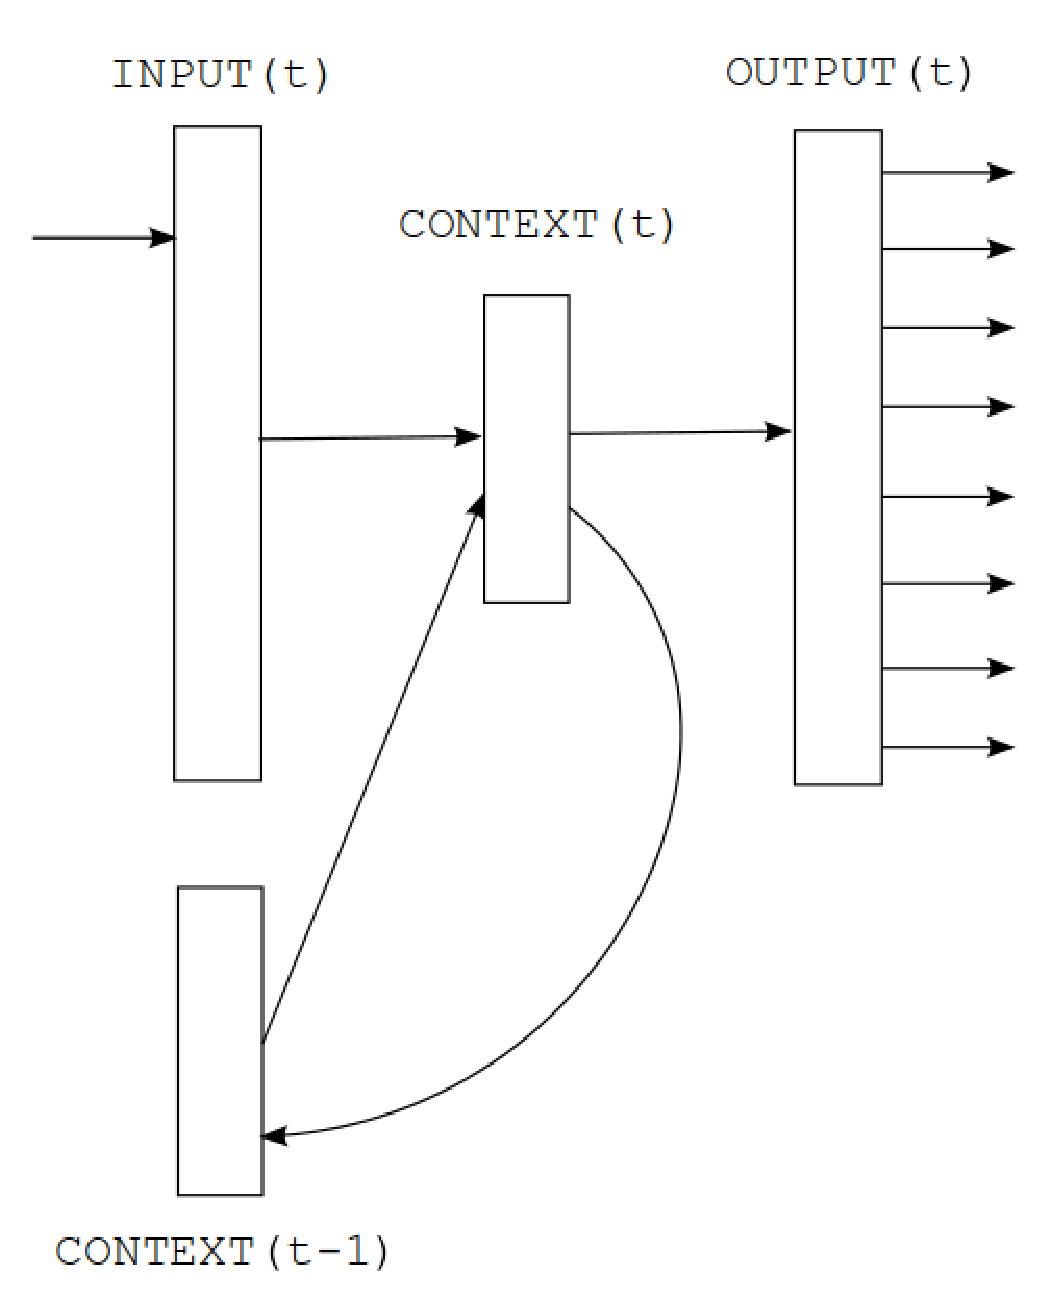
\includegraphics[width=70mm, height=70mm]{rnn.eps}
\caption{Simple Recurrent Neural Network(Figure from \cite{Mikolov:10}). \label{fig:rnn}}
\end{figure}

The architecture of a simple RNN consists of an input layer $x$, a hidden layer $s$(also known as context layer or network state) and an output layer $y$. Since the training is time dependent, we will denote input $x$ as $x(t)$, output $y$ as $y(t)$ and state $s$ as $s(t)$. Input vector $x(t)$ is a concatentaion of vector $w$ representing current word, and output from neurons in context layer $s$ at time $t-1$(We can also include output from context layer before $t-1$ as well). The equations of each layer are described below:
\begin{align}
x(t) = w(t) + s(t-1) \\
s_j(t) = f\bigg(\sum_{i}x_i(t)u_{ji}\bigg) \\
y_k(t) = g\bigg(\sum_{j}s_j(t)v_{kj}\bigg)
\end{align}
where $f(z)$ is sigmoid function for activation and $g(z)$ is a softmax function for output prediction:
\begin{align}
f(z) = \frac{1}{1+\mathrm{e}^{-z}} \\
g(z_m) = \frac{\mathrm{e}^{z_m}}{\sum_{k}\mathrm{e}^{z_k}}
\end{align}

\cite{Mikolov:10} claim that size of hidden layer reflects amount of training data with smaller size leading to less number of layers. Weights are initialized to random small values and updated using gradient descent. Output layer $y(t)$ represents probability distribution of next word given previous word $w(t)$ and context $s(t-1)$. The objective function is:
\begin{align}
error(t) =  actual(t) - y(t)
\end{align}
where $actual(t)$ is a $1$-hot vector representing the word that should have been predicted given the context.
\begin {table}[h!]
\centering
\begin{tabular}{ |c|c|c| }
\hline
Model & DEV WER & EVAL WER \\ \hline
Lattice 1 best & 12.9 & 18.4 \\ 
Baseline-KN5 (37M) & 12.2 & 17.2 \\
Discriminative LM (37M) & 11.5 & 16.9 \\
Joint LM (70M) (37M) & - & 16.7 \\ \hline
Static 3xRNN + KN5 (37M) & 11.0 & 15.5 \\
Dynamic 3xRNN + KN5 (37M) & 10.7 & 16.3 \\
\hline
\end{tabular}
\caption {Comparison of WSJ results obtained with various models(RNN is trained on just 6.4M words)}
\label{table:rnn}
\end{table}
Table \ref{table:rnn} representes results of \cite{Mikolov:10} obtained in WSJ experiments using RNN.\\

\cite{Mikolov:11} present several modifications of the original recurrent neural network language model (RNN LM). The present approaches that lead to more than 15 times speedup for both training and testing phases. They also show the importance of backpropagation through time(BPTT) which is an extension to backpropagation algorithm for recurrent networks. With truncated BPTT, the error is propagated through recurrent connections back in time for a specific number of time steps. Thus, the network learns to remember information for several time steps in the hidden layer when it is learned by the BPTT.\\
The speedup is obtained by assuming that words can be mapped to classes. Thus if we assume thate ach word belongs to exactly one class, we can first estimate the probability distribution over each class using RNN and then calculate the probability of a particular word from the desired class assuming unigram distribution of words within the class. Thus, now we are reducing the connections between hidden and output layer from $V$ to $C$ which is a significant improvement.\\
They are often very sensitive to small changes in its parameters which changes the gradient by a large amount. Few others are, Bi-directional RNN and Hierarchical RNN.\\

\section{Semantic Composition}
\label{sec:composition}
The Principle of Compositionality is that meaning of a complex expression is determined by the meaning of its parts or constituents and the rules which guide this combination. It is also known as \emph{Frege's Principle}. In our case, the constituents are word vectors and the expression in hand is the sentence/document vector. For example,
\begin{center}
\emph{The movie is funny and the screenplay is good}
\end{center}
In the above sentence, consider the word vectors are represented by $w(x)$ and the sentence vector as $S(x)$. Hence,
\begin{align}
S(x) = c_1w_1(x) \Theta c_2w_2(x) \Theta c_3w_3(x) \Theta c_4w_4(x) \dots \Theta c_kw_k(x)
\end{align}
where $\Theta$ can be any operation(e.g., addition, multiplication) and $c_i$s are constants.

\begin {table}[h!]
\centering
\begin{tabular}{ |c|c| }
\hline
Composition & Accuracy \\ \hline \hline
Average & 88.42 \\ \hline
Weighted Average & 88.41 \\ \hline
Multiplication & 50.30 \\ \hline
\end{tabular}
\caption {Results of Vector Composition with different Operations}
\label{table:composition}
\end{table}
Analyzing the results from Table \ref{table:composition}, we observed that when we deal with large number of features, there is a presence of large number of \emph{zeros} and presence of a single zero in a feature will make that features contribution zero in the final vector, which happens in our case and thus multiplicative composition fails.\\
We, therefore, adopt both simple and weighted average methods in our work. The advantage with addition is that, it doesnot increase the dimensionof the vector and captures high level semantics with ease. In fact, \cite{Zou:13} have used simple average to construct phrase vectors which they have later used to find phrase level similarity using cosine distance.\\
\cite{Mikolov:13c} showed that relations between words are reflected to a large extent in the offsets between their vector embeddings. They also use additive composition to reflect semantic dependencies.
\begin{center}
\emph{queen - king $\approx$ woman - man}
\end{center}
\cite{Blacoe:12} clearly show that vectors of Neural Language Model and Distributed Model when used with additive composition outperform those with multiplicative composition in Paraphrase Classification task. DM vectors outperform by nearly giving accuracy difference of 6\%. They also perfrom very well on Phrase simliarity tasks.\\
\cite{Socher:13} also present yet another model for semantic composition but that uses a sentiment treebank which is a very costly structure to build and it is task dependent. For under-resourced languages such as Hindi, it would take years to build (for English, task done through Amazaon Mechanical Turk). This leads to appreciation of models such as Additive Composition.\\
\begin{figure}[ht!]
\centering
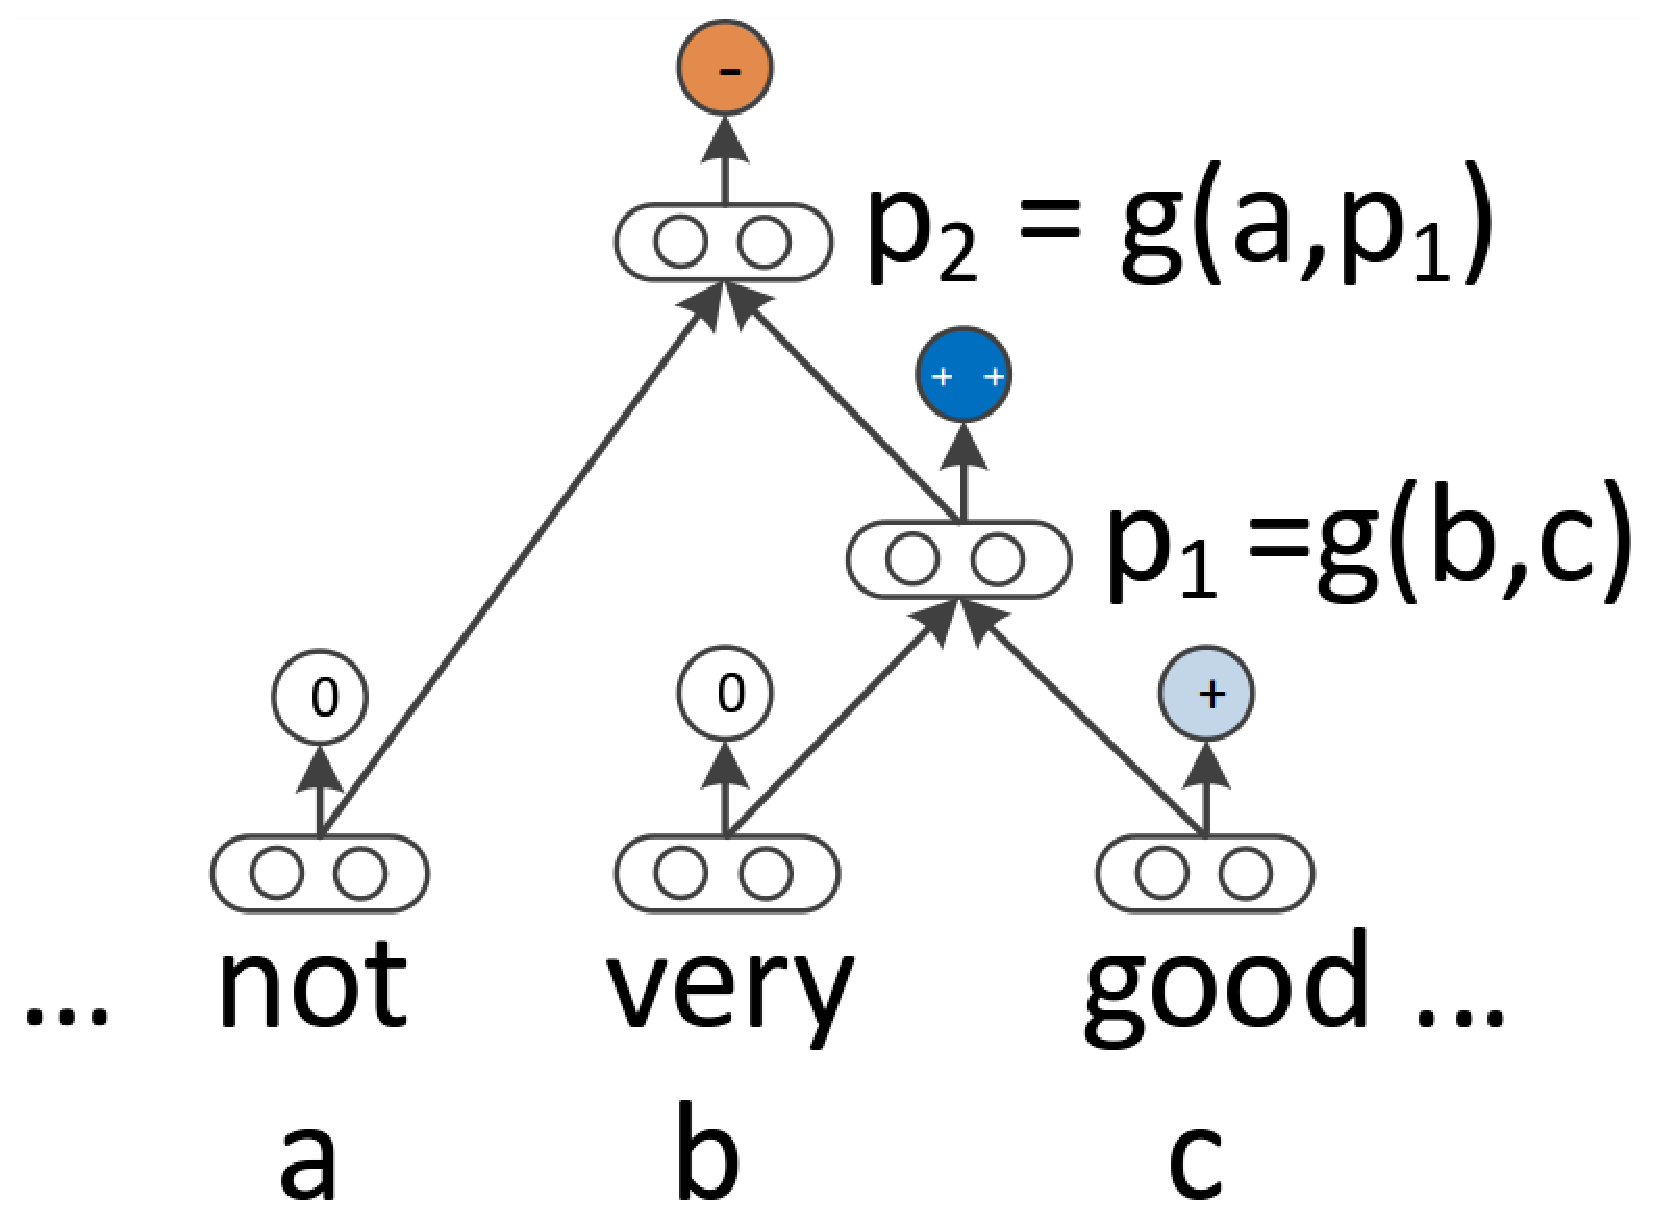
\includegraphics[width=90mm, height=80mm]{recursiveNN.eps}
\caption{Approach of Recursive Neural Network(Figure from \cite{Socher:13}). \label{fig:recursiveNN}}
\end{figure}
Figure \ref{fig:recursiveNN} depicts the approach of recursive neural network. When an n-gram is given to the compositional models, it is parsed into a binary tree and each leaf node, corresponding to a word, is represented as a vector. Recursive neural models will then  compute parent vectors in a bottom up fashion using different types of compositionality functions $g$. The parent vectors are again given as features to a classifier.

